\documentclass[preprint,12pt]{elsarticle}

\usepackage{amsmath,amssymb}
\usepackage{graphicx}
\usepackage{booktabs}
\usepackage{tabularx}
\usepackage{array}
\usepackage{xcolor}
\usepackage{xurl}
\usepackage{hyperref}
\usepackage{algorithm}
\usepackage{algpseudocode}
\usepackage{tikz}
\usetikzlibrary{positioning,arrows.meta,fit,backgrounds}
\usepackage{lineno}

\journal{Computers, Environment and Urban Systems}
\bibliographystyle{elsarticle-num}

%% ---------------------------------------------------------------------------
%% Every result quoted in this manuscript is a macro written by
%%   pimaluos report --results results/paper --out paper/generated
%% Before that command has been run, the macros render as [TBD].
%% ---------------------------------------------------------------------------
\IfFileExists{generated/macros.tex}{\def\GenDir{generated}}{\def\GenDir{pending}}
\input{\GenDir/macros.tex}
\makeatletter\newcommand{\Rows}[1]{\@@input \GenDir/#1.tex }\makeatother
\newcommand{\FigOr}[2]{\IfFileExists{#1}{\includegraphics[#2]{#1}}{%
  \fbox{\parbox{0.8\linewidth}{\centering\vspace{2em}\textbf{[TBD]} figure written by \texttt{pimaluos report}\vspace{2em}}}}}
%% Notes for the author; remove all \AuthorNote before submission.
\newcommand{\AuthorNote}[1]{\par\noindent\fcolorbox{red}{red!5}{\parbox{0.97\linewidth}{\small\textbf{Author note:} #1}}\par}
\newcommand{\cotwo}{CO$_2$e}

\begin{document}

\begin{frontmatter}

\title{Context over prescription: stakeholder agents and many-objective search for lot-level land-use plans that balance social, economic and environmental outcomes}

\author[uwm]{Parya Payami\corref{cor1}}
\ead{ppayami@uwm.edu}
\cortext[cor1]{Corresponding author}
\affiliation[uwm]{organization={School of Architecture and Urban Planning, University of Wisconsin--Milwaukee},
  city={Milwaukee}, state={WI}, country={USA}}

\begin{abstract}
Universal planning paradigms such as the 15-minute city prescribe one urban form for every place, while zoning decisions are taken lot by lot, by actors with unequal power, in cities that already differ widely in what they lack. We present PIMALUOS, an open-source framework that plans added floor area by use (residential, office, retail, community facility) for every lot of a city and evaluates each plan jointly on social, economic and environmental outcomes rather than as a sequence of single-issue checks. Plans are bounded by the zoning envelope in force, including New York City's 2024 City of Yes Universal Affordability Preference and Mandatory Inclusionary Housing. One vectorised outcome model computes homes and income-restricted homes, per-capita access to six everyday destination categories within a 15-minute walk on the street network, jobs, property tax, jobs--housing balance, land-use mix, 30-year life-cycle carbon, transit orientation, flood exposure and floor area added on displacement-vulnerable lots, together with traffic, sewer and sunlight screens. Five stakeholder agents (residents, developers, planners, environmental and equity advocates), trained with proximal policy optimisation on parcel-graph embeddings, vote on every lot; their awareness of city-wide outcomes is a parameter. NSGA-III searches the same space on eight objectives, and a Monte Carlo analysis tests whether comparisons survive parameter uncertainty. On \NParcels{} Manhattan lots (MapPLUTO \PlutoRelease{}), the verified PIMALUOS plan adds \PimHomesKVer{} thousand homes (\PimAffHomesKVer{} thousand income-restricted) and \PimJobsKVer{} thousand jobs, moves the access index from \BaseAccess{} to \PimAccessVer{} and emits \PimCarbonMtVer{} Mt~\cotwo{} over 30 years; the verified as-of-right build-out with the affordability preference adds \BoUapHomesKVer{} thousand homes and \BoUapJobsKVer{} thousand jobs at an access index of \BoUapAccessVer{} and \BoUapCarbonMtVer{} Mt~\cotwo{}. Every number is regenerated from public data by one command.
\end{abstract}

\begin{highlights}
\item Lot-level plans by use, evaluated jointly on social, economic and environmental goals
\item Per-capita 15-minute access on the street network instead of a binary proximity target
\item Zoning envelope includes City of Yes affordability preference and inclusionary housing
\item Five stakeholder agents with tunable city-wide awareness vote on every Manhattan lot
\item Eight-objective search and Monte Carlo uncertainty test every comparison
\end{highlights}

\begin{keyword}
land-use planning \sep 15-minute city \sep accessibility \sep multi-agent reinforcement learning \sep many-objective optimisation \sep embodied carbon \sep affordable housing \sep zoning
\end{keyword}

\end{frontmatter}

\linenumbers

%% ===========================================================================
\section{Introduction}
%% ===========================================================================

Planning theory has long warned against universal models of the good city. Garden cities, the towers-in-the-park of high modernism, transit-oriented development and, most recently, the 15-minute city \cite{moreno2021fifteen} each began as a response to particular problems in particular places, and each was later applied as a template elsewhere \cite{scott1998seeing}. The 15-minute city illustrates the risk well. Its aim, that everyday needs be reachable on foot or by bicycle, is widely shared, but recent reviews show that a proximity target says little about the capacity of the services reached, who can afford to live near them, whether residents choose to use them, or how proximity interacts with jobs and regional travel \cite{mouratidis2024time,mahmoudpour2026critical}. In dense cores such as Manhattan almost every resident already lives within 15 minutes of every everyday destination category, yet services there can still be scarce \emph{per person}, and homes near them can still be unaffordable. What a place needs depends on its context: more housing in one neighbourhood, a school in another, jobs near homes in a third.

Planning is also a contest between actors with unequal power. Built form can frame and reproduce power relations without anyone stating them \cite{dovey1999framing}; rationality in planning is shaped by power \cite{flyvbjerg1998rationality}; and who decides the shape of the city is a question of rights \cite{harvey2008right} and of justice \cite{fainstein2010just}. Participation ranges from consultation that leaves decisions unchanged to genuine delegation of power \cite{arnstein1969ladder}. Computational planning tools are not neutral either: they encode whose objectives count and how much \cite{townsend2013smart}. A tool that is to support context-sensitive planning should therefore make three things explicit and adjustable: what each stakeholder wants, how their preferences are combined, and how a plan performs on every goal, social, economic and environmental, at once.

Existing tools address parts of this agenda. Multi-objective land-use allocation trades off aggregate objectives over grid cells \cite{stewart2004genetic,cao2011spatial,sicuaio2024sustainable}; game-theoretic and agent-based models represent stakeholders and their negotiation \cite{abolhasani2022collective}; and learned planners generate land-use layouts with adversarial, reinforcement or language-model agents \cite{wang2020reimagining,zheng2023spatial,qian2023aiagent,zhou2024llm}. Qian et al.\ \cite{qian2023aiagent} in particular let stakeholder agents with graded awareness of the wider city vote on land-use readjustment. These studies use stylised or small study areas, a single land-use label per cell, and outcome indicators that are mostly computed after the fact rather than used to train and constrain the planner; none couples stakeholder agents to street-network accessibility, the jobs--housing balance, carbon and infrastructure capacity on real parcels under current zoning.

We present PIMALUOS, an open-source framework that does this for every lot of a borough. The decision is how much floor area each lot adds in each of four uses, within the zoning envelope in force. Every plan is evaluated by one outcome model that covers the three pillars together (Table~\ref{tab:goals}); there are no separate ``15-minute'', ``mix'' or ``jobs--housing'' phases. Accessibility is measured as per-capita supply within a 15-minute walk \cite{luo2003measures}, so that adding homes near a saturated clinic lowers access and adding a clinic where none is within reach raises it. Stakeholder agents learn from these outcomes, and NSGA-III searches the same space as a non-negotiated reference. We apply the framework to Manhattan under the zoning adopted in City of Yes for Housing Opportunity (2024) and the Midtown South Mixed-Use Plan (2025) \cite{nyc_coy2024,nyc_msmx2025}.

The contributions are:
\begin{enumerate}
\item an integrated, vectorised outcome model for lot-level, use-specific plans that computes social, economic and environmental indicators and infrastructure screens for a whole borough in well under a second, so that it can serve as the learning signal, the search objective and the verification of every plan;
\item a multi-agent formulation in which five stakeholder utilities defined on those outcomes are learned with PPO, combined by an explicit voting rule whose game-theoretic properties are analysed, with stakeholder awareness and voting power as parameters rather than hidden assumptions;
\item an evaluation on all of Manhattan against as-of-right build-outs with and without the affordability preference, rule-based growth, ablations and eight-objective NSGA-III fronts, with a Monte Carlo test of whether each comparison survives parameter uncertainty;
\item an open, tested package that rebuilds every number, table and figure in this paper from public data with recorded checksums.
\end{enumerate}

\begin{table}[t]
\centering\small
\caption{Goals evaluated for every plan, by pillar. All are computed by the same outcome model (Section~\ref{sec:outcomes}); none is a separate design phase.}
\label{tab:goals}
\begin{tabularx}{\linewidth}{>{\raggedright\arraybackslash}p{0.2\linewidth}X}
\toprule
Pillar & Indicators \\
\midrule
Social & homes; income-restricted homes (UAP, MIH); per-capita access to food, health care, education, parks, civic and cultural facilities and transit within a 15-minute walk; share of residents with all six within 15 minutes; floor area added on displacement-vulnerable lots \\
Economic & jobs; annual property tax; market value; jobs--housing balance and land-use mix within the 15-minute walkshed \\
Environmental & embodied, operational and 30-year life-cycle carbon; share of new floor area within a 15-minute walk of a subway station; floor area added in flood zones; newly shaded lots \\
Capacity & peak-hour traffic and combined-sewer load relative to existing capacity \\
\bottomrule
\end{tabularx}
\end{table}

%% ===========================================================================
\section{Related work}
%% ===========================================================================

\paragraph{Land-use optimisation} Multi-objective land-use allocation with evolutionary algorithms assigns land-use classes to cells under aggregate objectives \cite{stewart2004genetic,cao2011spatial}; recent work adds sustainability and resilience objectives \cite{sicuaio2024sustainable}. Stakeholders appear, if at all, as objective weights. We keep this tradition as our NSGA-III reference \cite{deb2014nsga3,blank2020pymoo}.

\paragraph{Stakeholders, games and learned planners} Abolhasani et al.\ \cite{abolhasani2022collective} simulate collective land-use decisions as a game among event-driven actors. Wang et al.\ \cite{wang2020reimagining} generate land-use configurations with adversarial learning; Zheng et al.\ \cite{zheng2023spatial} lay out land use and roads with deep reinforcement learning on graphs; Qian et al.\ \cite{qian2023aiagent} let stakeholder agents vote on land-use readjustment, and introduce agents whose rewards weigh their own parcel against the whole city; Zhou et al.\ \cite{zhou2024llm} let language-model agents role-play residents in participatory planning. PIMALUOS adopts the voting and awareness ideas but applies them to floor area by use on all lots of a borough, couples agents to network-based outcomes and infrastructure screens, and treats the voting rule as an object of analysis (Table~\ref{tab:positioning}).

\paragraph{Accessibility, the 15-minute city and its critics} The 15-minute city \cite{moreno2021fifteen} builds on decades of work linking density, diversity and design to travel \cite{ewing2010travel}, jobs--housing balance \cite{cervero1989jobs} and land-use mix \cite{song2013comparing}. Reviews published in 2024--2026 identify recurring pitfalls: binary proximity thresholds ignore capacity and quality, mixed use can raise land values and displace residents, and local self-sufficiency can neglect access to regional jobs \cite{mouratidis2024time,mahmoudpour2026critical}. We respond to each: access is per-capita supply (two-step floating catchment area, 2SFCA \cite{luo2003measures}), displacement exposure is an explicit objective, and jobs--housing balance is evaluated alongside local access.

\paragraph{Graph learning for cities} Graph neural networks are widely used for urban prediction \cite{jin2024spatio,jiang2022graph,wang2022deep} and land-use sensing \cite{yao2017sensing}. We use relation-aware graph attention \cite{velickovic2018gat,wang2019han} pre-trained by masked-feature reconstruction \cite{hou2022graphmae}, implemented in PyTorch Geometric \cite{fey2019pyg,paszke2019pytorch}; agents are trained with PPO \cite{schulman2017ppo,schulman2016gae,yu2022mappo}; see \cite{zhang2021marl} for an overview of multi-agent reinforcement learning and \cite{chu2020marl} for an urban application.

\paragraph{Digital twins and transparency} Urban digital twins promise to evaluate interventions before they are built \cite{batty2018digital,albalkhy2024digital}; open toolkits for networks \cite{boeing2017osmnx,sevtsuk2025madina}, imagery \cite{ito2025zensvi,mahajan2024greenr}, microsimulation \cite{waddell2002urbansim} and interactive planning tables \cite{alonso2018cityscope} make parts of this possible. PIMALUOS is not a real-time twin; it is a reproducible scenario engine whose assumptions are tabulated and whose parameters, including stakeholder power, can be changed and re-run.

\begin{table}[t]
\centering\small
\caption{Positioning of PIMALUOS relative to representative work.}
\label{tab:positioning}
\begin{tabularx}{\linewidth}{>{\raggedright\arraybackslash}p{0.2\linewidth}>{\raggedright\arraybackslash}X>{\raggedright\arraybackslash}X>{\raggedright\arraybackslash}X}
\toprule
Work & Decision & Method & Stakeholders / outcomes \\
\midrule
\cite{stewart2004genetic,cao2011spatial,sicuaio2024sustainable} & Land-use class per cell & Genetic / NSGA-II & Aggregate objectives \\
\cite{abolhasani2022collective} & Land-use change & Game theory, event-driven actors & Negotiating actors \\
\cite{wang2020reimagining} & Land-use configuration & Adversarial learning & -- \\
\cite{zheng2023spatial} & Land use and roads & Deep RL on graphs & Single planner; service coverage \\
\cite{qian2023aiagent} & Land-use readjustment & Consensus MARL with GNN & Voting agents with awareness levels \\
\cite{zhou2024llm} & Land-use plan & LLM role-play agents & Simulated residents' satisfaction \\
PIMALUOS & Added floor area by use per lot (whole borough, current zoning) & GAT + PPO agents + voting; NSGA-III; Monte Carlo & Five agents; social, economic, environmental outcomes and capacity screens \\
\bottomrule
\end{tabularx}
\end{table}

%% ===========================================================================
\section{Data and study area}\label{sec:data}
%% ===========================================================================

\paragraph{Parcels and zoning} We use MapPLUTO release \PlutoRelease{} \cite{dcp_mappluto}, restricted to Manhattan (BoroCode 1) and projected to EPSG:2263 (US feet). Of \NParcelsRaw{} lots, \NParcels{} with positive lot area are used. This release records the zoning adopted in City of Yes for Housing Opportunity (5 December 2024) \cite{nyc_coy2024}, including the Universal Affordability Preference (UAP), which allows residential floor area above the market-rate maximum (ResidFAR) up to AffResFAR if the additional floor area is income-restricted, and the Midtown South Mixed-Use Plan (14 August 2025) \cite{nyc_msmx2025}, which mapped residential districts with FAR up to 18 in former manufacturing areas. Lots in Mandatory Inclusionary Housing (MIH) areas (\NMihLots{} lots) must set aside \MihShare{}\,\% of residential floor area as income-restricted (Option~1, ZR~23-154 \cite{nyc_zr}). Existing floor area is \ExistingFAM{} million sq\,ft. The zoning envelope (Section~\ref{sec:envelope}) allows \CapTotalM{} million sq\,ft of additional floor area in total: \CapResMarketM{} million residential at market rate, \CapResUapM{} million residential with the UAP, \CapComM{} million commercial and \CapFacM{} million community facility (use capacities overlap and are not additive). \LotsAboveMax{} lots already exceed their zoning maximum.

\paragraph{Context data} Table~\ref{tab:sources} lists the other public sources. The walking network is the NYC street centreline restricted to walkable segments (\WalkNodes{} nodes in the largest connected component); a 15-minute walk is \WalkMinutes{} minutes at 80~m/min, i.e.\ 1{,}200~m of network distance, and reaches \WalkshedNodes{} nodes on average. Destinations are \DestFood{} food stores, \DestHealth{} hospitals and clinics, \DestEducation{} schools and child-care sites, \DestParksAcres{} acres of parks, \DestCivic{} libraries, community and cultural centres and \DestTransit{} subway stations. Lots hold \PopTotalM{} million residents (2020 Census blocks, allocated to lots by residential units) and \JobsTotalM{} million jobs (LODES 2023 workplace characteristics, allocated by commercial floor area); \WorkersTotalK{} thousand employed residents (LODES residence characteristics) live in Manhattan.

\begin{table}[t]
\centering\small
\caption{Public data sources. The file name, URL, retrieval date and SHA-256 checksum of every download are recorded in \url{results/paper/context_manifest.json}.}
\label{tab:sources}
\begin{tabularx}{\linewidth}{>{\raggedright\arraybackslash}p{0.3\linewidth}>{\raggedright\arraybackslash}X}
\toprule
Source & Use \\
\midrule
MapPLUTO 26v2 \cite{dcp_mappluto} & lots, zoning (ResidFAR, AffResFAR, CommFAR, FacilFAR, ManuFAR, MIH), floor area by use, assessed value, flood zones \\
Street Centreline (CSCL) \cite{nyc_cscl} & walking network \\
Facilities Database \cite{nyc_facdb} & health, education, civic destinations \\
Retail Food Stores \cite{nys_food} & food destinations and floor area \\
Parks Properties \cite{nyc_parks} & park access points and area \\
MTA Subway Stations \cite{mta_stations} & transit destinations \\
2020 Census P.L.\ 94-171 \cite{census2020pl} & block population \\
LODES 8, 2023 \cite{lodes8} & jobs (WAC) and employed residents (RAC) by block \\
CLF WBLCA v2 \cite{benke2025harmonized,clf_wblca_data} & embodied carbon of new construction by use \\
LL84 benchmarking 2024 \cite{nyc_ll84} & operational carbon of recent buildings by use \\
NYC DOF FY2026 \cite{nyc_dof2026} & tax rates and assessment ratios \\
\bottomrule
\end{tabularx}
\end{table}

\paragraph{Existing conditions} Before any change, \BaseFullPct{}\,\% of residents live within 15 minutes of all six destination categories: Manhattan already ``is'' a 15-minute city in the binary sense, which is why we measure access per capita. The resident-weighted access index (Section~\ref{sec:outcomes}) is \BaseAccess{} (1 would mean every category at the borough median supply per person), the mean jobs--housing balance within walking distance is \BaseJH{} and the mean land-use mix is \BaseMix{}.

\paragraph{Node features} Lot features are engineered from MapPLUTO (geometry, built form, regulation, assessed value, distance to open space and to Grand Central, land-use one-hot) and from the context data (population and job density, walking minutes to each destination category, existing access index, jobs--housing balance and land-use mix). Heavy-tailed variables are log-transformed and all are standardised; constant features are dropped, leaving \NFeatures{} of \NFeaturesEngineered{} (\ref{app:features}).

%% ===========================================================================
\section{Methods}
%% ===========================================================================

\begin{figure}[t]
\centering
\resizebox{\linewidth}{!}{%
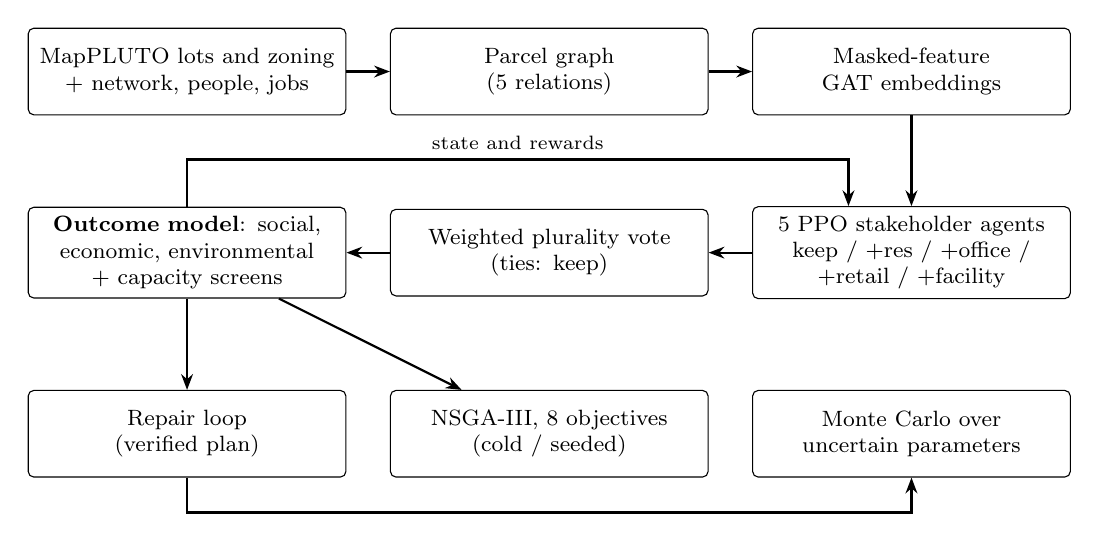
\begin{tikzpicture}[every node/.style={font=\footnotesize},
  box/.style={draw, rounded corners=2pt, align=center, minimum height=11mm, text width=38mm, fill=white},
  arr/.style={-{Stealth[length=2mm]}, thick}]
\node[box] (data) at (0,0) {MapPLUTO lots and zoning\\+ network, people, jobs};
\node[box] (graph) at (4.6,0) {Parcel graph\\(5 relations)};
\node[box] (enc) at (9.2,0) {Masked-feature\\GAT embeddings};
\node[box] (out) at (0,-2.3) {\textbf{Outcome model}: social,\\economic, environmental\\+ capacity screens};
\node[box] (vote) at (4.6,-2.3) {Weighted plurality vote\\(ties: keep)};
\node[box] (agents) at (9.2,-2.3) {5 PPO stakeholder agents\\keep / +res / +office /\\+retail / +facility};
\node[box] (repair) at (0,-4.6) {Repair loop\\(verified plan)};
\node[box] (nsga) at (4.6,-4.6) {NSGA-III, 8 objectives\\(cold / seeded)};
\node[box] (mc) at (9.2,-4.6) {Monte Carlo over\\uncertain parameters};
\draw[arr] (data) -- (graph);
\draw[arr] (graph) -- (enc);
\draw[arr] (enc) -- (agents);
\draw[arr] (agents) -- (vote);
\draw[arr] (vote) -- (out);
\draw[arr] (out) -- (repair);
\draw[arr] (out) -- (nsga);
\draw[arr] (repair) -- ++(0,-1.0) -| (mc);
\draw[arr] (out.north) -- ++(0,0.6) -| node[pos=0.25, above, font=\scriptsize]{state and rewards} ([xshift=-8mm]agents.north);
\end{tikzpicture}}
\caption{PIMALUOS. One outcome model provides the agents' state and rewards, the NSGA-III objectives and the verification of every plan.}
\label{fig:architecture}
\end{figure}

\subsection{Plans and the zoning envelope}\label{sec:envelope}
A plan $X\in\mathbb{R}_{\ge0}^{N\times4}$ gives the floor area (sq\,ft) each lot $i$ adds in residential, office, retail and community-facility use, $X_i=(x^{r}_i,x^{o}_i,x^{t}_i,x^{f}_i)$. Existing floor area is never removed. With lot area $A_i$, existing residential, commercial and facility floor area $R^0_i,C^0_i,F^0_i$ and existing FAR $f^0_i$, the envelope is
\begin{equation}
\begin{aligned}
x^r_i &\le \bar R_i = \max(0,\ \mathrm{AffResFAR}_i A_i - R^0_i),\\
x^o_i + x^t_i &\le \bar C_i = \max(0,\ \mathrm{CommFAR}_i A_i - C^0_i),\\
x^f_i &\le \bar F_i = \max(0,\ \mathrm{FacilFAR}_i A_i - F^0_i),\\
\textstyle\sum_u x^u_i &\le \bar T_i = (\bar u_i - f^0_i) A_i,
\end{aligned}
\end{equation}
with $\bar u_i=\max(\mathrm{AffResFAR}_i,\mathrm{CommFAR}_i,\mathrm{FacilFAR}_i,\mathrm{ManuFAR}_i,f^0_i)$ (the use maxima are alternatives, not additive). Plans outside the envelope are projected into it by clipping each use, scaling office and retail proportionally to $\bar C_i$ and scaling all uses to $\bar T_i$. Residential floor area above the market-rate capacity $\bar R^{m}_i=\max(0,\mathrm{ResidFAR}_iA_i-R^0_i)$ is income-restricted (UAP), and in MIH areas a share $m=\MihShare{}\,\%$ of market-rate floor area is too:
\begin{equation}
a_i = \max(0,\ x^r_i - \bar R^m_i) + m\,\mathbb{1}[\mathrm{MIH}_i]\min(x^r_i,\bar R^m_i).
\end{equation}
Zoning compliance therefore holds by construction for every plan. MapPLUTO does not record other bonuses or special-district rules, which are not modelled.

\subsection{Outcome model}\label{sec:outcomes}
All outcomes are computed for the whole borough in one vectorised pass (about 0.07~s for Manhattan). Lots are attached to their nearest walking-network node; $\mathbf R$ is the sparse node-to-node matrix with $R_{vw}=1$ if $w$ is within a 15-minute walk of $v$.

\paragraph{Homes, people and jobs} New homes are $x^r_i/s$ with $s=\UnitSqft{}$~sq\,ft, the median floor area per unit of Manhattan residential buildings completed since 2010; new residents are homes times \PersonsPerUnit{} persons per unit (2020 Census population over MapPLUTO units), of whom a share \EmployedPerResident{} is employed (LODES RAC over population). New jobs are $\sum_u \rho_u x^u_i$, with jobs per 1{,}000~sq\,ft $\rho_o=\JobsKsfOffice{}$, $\rho_t=\JobsKsfRetail{}$, $\rho_f=\JobsKsfFacility{}$ estimated by non-negative least squares of LODES 2023 block jobs on block floor area by use ($R^2=\JobsModelRsq{}$).

\paragraph{Per-capita 15-minute access} For each category $k$ (food, health, education, parks, civic, transit) and node $w$, supply $S_{wk}$ is food-store floor area, clinics and hospitals, enrolment seats, park acres, civic sites or stations. New retail adds daily-needs supply in proportion to its floor area (share $\DailyNeedsSharePct{}\,\%$, the ratio of food-store to retail floor area today); new community-facility floor area adds sites (one per \FacilitySqftPerSite{}~sq\,ft, the existing ratio) of the service category that is least supplied at that node. With node population $P_w$ (existing plus new residents), the 2SFCA \cite{luo2003measures} supply per person reachable from node $v$ is
\begin{equation}
\mathrm{Acc}_{vk} = \sum_w R_{vw}\, \frac{S_{wk}}{\sum_{v'} R_{wv'} P_{v'}},
\end{equation}
and the access index is the geometric mean over categories relative to the existing resident-weighted median $\tilde{\mathrm{Acc}}_k$, averaged over residents geometrically:
\begin{equation}
\mathrm{AI}=\exp\Big(\sum_v \frac{P_v}{\sum P}\ \frac1K\sum_k \log\frac{\mathrm{Acc}_{vk}}{\tilde{\mathrm{Acc}}_k}\Big).
\end{equation}
Adding residents near fixed services lowers AI; adding services where demand is high raises it. We also report the share of residents with every category within 15 minutes (binary proximity), for comparison with the conventional 15-minute metric.

\paragraph{Jobs--housing balance and mix} Within each walkshed, with jobs $J$ and employed residents $W$, balance is $\min(J,W)/\max(J,W)\in[0,1]$ \cite{cervero1989jobs}, averaged over residents and jobs; mix is the normalised entropy of residential, office, retail and facility floor area \cite{song2013comparing}, averaged over residents.

\paragraph{Fiscal and market value} Annual property tax is market-rate residential floor area times the local median assessed value per sq\,ft of residential lots (within the traffic cell; borough median where none) times the class~2 rate (\TaxRateTwo{} per \$100 AV), plus office and retail floor area times the commercial median and the class~4 rate (\TaxRateFour{}) \cite{nyc_dof2026}. Income-restricted floor area is assumed tax-exempt. Market value divides assessed value by the assessment ratio (0.45), valuing income-restricted floor area at a factor \AffValueFactor{} of market-rate value.

\paragraph{Carbon} Embodied carbon (life-cycle stages A--C, kg~\cotwo{}/m$^2$) is the median of new buildings of the corresponding use in the CLF WBLCA v2 dataset \cite{benke2025harmonized,clf_wblca_data}: residential \EciRes{} ($n=\EciResN{}$), office \EciOffice{} ($n=\EciOfficeN{}$), retail \EciRetail{} and community facility \EciFacility{} ($n=\EciFacilityN{}$). Operational carbon (kg~\cotwo{}/sq\,ft/yr) is the median of location-based emissions per floor area of Manhattan buildings completed since 2010 in the 2024 LL84 benchmarking data \cite{nyc_ll84}: residential \OpcRes{} ($n=\OpcResN{}$), office \OpcOffice{} ($n=\OpcOfficeN{}$), retail \OpcRetail{} ($n=\OpcRetailN{}$), facility \OpcFacility{} ($n=\OpcFacilityN{}$). Life-cycle carbon is embodied plus \LifecycleYears{} years of operational carbon, with today's grid; the Local Law~97 limits \cite{nyc_ll97} and grid decarbonisation would reduce the operational part, so these figures are upper bounds for operation. The \emph{transit-oriented share} is the share of added floor area within a 15-minute walk of a subway station; \emph{flood exposure} is floor area added on lots in the 2007 or 2015 FEMA 1\,\% flood zones recorded in MapPLUTO.

\paragraph{Displacement exposure} Lots are \emph{vulnerable} if they hold residential units and are in the bottom quartile of assessed value per unit (\NVulnerable{} lots) \cite{chapple2016forewarned,bartik2023costs}; the indicator is floor area added on them. No tenure, rent or demographic data are used, so this is a proxy for pressure on lower-cost housing, not a measure of who is displaced.

\paragraph{Capacity screens} Three planning-scale screens (Table~\ref{tab:params}) flag stress on infrastructure and neighbours. \emph{Traffic}: peak-hour vehicle trips (rates per 1{,}000 sq\,ft by use) are summed over 1{,}320~ft cells whose capacity is proportional to street frontage, calibrated so that the median existing volume-to-capacity ratio is 0.7 and floored so that existing demand is served (frontage alone left \ExistingTazOverRaw{} of \NTaz{} cells over capacity today); a cell whose V/C exceeds 1 and increases is a violation \cite{bpr1964traffic}. \emph{Sewer}: peak combined load per 2{,}640~ft catchment (\NCatch{} catchments) is Rational-Method storm flow \cite{kuichling1889relation} plus peaked sanitary flow proportional to floor area; a catchment above existing load plus 10\,\% headroom is a violation. \emph{Sunlight}: at winter-solstice noon a building casts a shadow of length $H/\tan(90^\circ-\varphi-23.44^\circ)$ due north; lots shaded in the plan but not today are \emph{newly shaded} \cite{knowles2003solar}. Because capacities are calibrated to existing conditions, only relative stress is meaningful.

\begin{table}[t]
\centering\small
\caption{Capacity-screen parameters (defaults in \texttt{CapacityParams}). They are planning assumptions, not calibrated estimates; trip rates are informed by, not taken from, \cite{ite2021trip}.}
\label{tab:params}
\begin{tabularx}{\linewidth}{>{\raggedright\arraybackslash}p{0.42\linewidth}X}
\toprule
Parameter & Value \\
\midrule
Floor height; maximum coverage & 11 ft; 0.80 \\
Traffic cell; catchment cell & 1{,}320 ft; 2{,}640 ft \\
Reference median V/C; violation threshold & 0.70; 1.00 \\
Peak vehicle trips per 1{,}000 sq\,ft (added) & residential 0.15, office 0.50, retail 0.50, community facility 0.30 \\
Rainfall intensity; roof $C$; paved $C$ & 1.75 in/h; 0.95; 0.85 \\
Sanitary flow; peaking factor; sewer headroom & $2\times10^{-4}$ cfs per 1{,}000 sq\,ft; 2.5; 10\,\% \\
Shadow candidates per lot; latitude & 24; 40.78$^\circ$ \\
\bottomrule
\end{tabularx}
\end{table}

\begin{table}[t]
\centering\small
\caption{Outcome-model parameters as used in the run (written by \texttt{pimaluos report}).}
\label{tab:outparams}
\begin{tabularx}{\linewidth}{>{\raggedright\arraybackslash}p{0.44\linewidth}r>{\raggedright\arraybackslash}X}
\toprule
Parameter & Value & Source \\
\midrule
\Rows{tab_params_rows}
\bottomrule
\end{tabularx}
\end{table}

\subsection{Verification and repair}
Algorithm~\ref{alg:repair} removes added floor area that causes traffic, sewer or sunlight violations. It is applied to every plan, including baselines, so that all plans are compared after verification on equal terms. Repair only shrinks additions and existing conditions have no violations, so it terminates.

\begin{algorithm}[t]
\caption{Verification and repair}\label{alg:repair}
\begin{algorithmic}[1]
\State project $X$ into the envelope; $t\gets0$
\Loop
  \State evaluate screens; \textbf{if} no violations \textbf{then return} $X$
  \State $B\gets$ lots adding floor area in a violating cell or catchment, or newly shading a lot
  \State \textbf{if} $B=\emptyset$ \textbf{then return} $X$
  \State $\rho \gets 0.5$ if $t<30$ else $0$; \quad $X_B \gets \rho X_B$; \quad $t\gets t+1$
\EndLoop
\end{algorithmic}
\end{algorithm}

\subsection{Parcel graph and encoder}
All lots are nodes; five relations are built, symmetrised and de-duplicated (Table~\ref{tab:graph}): spatial adjacency (boundaries within 1~ft, weighted by shared length over perimeter), proximity ($k=8$ nearest lots within 300~ft), functional similarity (those pairs with the same land use), street frontage (two nearest lots on the same street within 600~ft) and regulatory coupling (five nearest lots in the same zoning district within 1{,}000~ft). Each of two encoder layers applies a relation-specific graph attention convolution \cite{velickovic2018gat} with four heads and combines relations with semantic attention \cite{wang2019han},
\begin{gather}
\tilde h_i = \sum_{r} \beta_r\, z^{(r)}_i,\qquad z^{(r)}_i=\mathrm{GAT}_r(h, E_r)_i,\\
\beta_r = \operatorname*{softmax}_{r}\Big(\tfrac{1}{N}\textstyle\sum_{i} q^\top \tanh\big(W z^{(r)}_i\big)\Big),
\end{gather}
followed by a residual connection, layer normalisation, ELU and dropout ($p=0.2$), and a projection to 128 dimensions (hidden width 256). The encoder is pre-trained by masked-feature reconstruction \cite{hou2022graphmae}: each epoch 15\,\% of training nodes are replaced by a learned mask token and reconstructed. Ten per cent of nodes are held out; we keep the parameters with the lowest held-out error (AdamW, learning rate $10^{-3}$, cosine decay, \GnnEpochs{} epochs).

\begin{table}[t]
\centering\small
\caption{Parcel graph: directed edges stored and unique undirected relations.}
\label{tab:graph}
\begin{tabular}{lrr}
\toprule
Relation & Directed & Undirected \\
\midrule
\Rows{tab_graph_rows}
\bottomrule
\end{tabular}
\end{table}

\subsection{Stakeholder agents}
At each of $H=\MarlHorizon{}$ steps, every lot receives one of five actions: keep, or add $\delta A_i$ (with $\delta=0.5$ FAR) of residential, office, retail or community-facility floor area, projected into the envelope. Each stakeholder type has one actor--critic policy (two hidden layers of 64 units) shared over all lots. A lot's state is its embedding and 14 dynamic signals: the used share of its total, residential, commercial and facility capacity; its cell's V/C; its catchment's sewer utilisation; the lots it newly shades; per-capita access, jobs--housing balance and mix in its walkshed; and indicators for transit within 15 minutes, flood zone, vulnerability and MIH. All five agents propose an action for every lot; the proposals are aggregated by weighted plurality (equal weights 0.2), with ties resolved to ``keep''.

Utilities are defined on the outcome model, per lot. Floor-area terms are in FAR units, and money and carbon are scaled by borough medians so that one FAR of typical floor area is about one unit:
\begin{align}
U^{\text{res}}_i &= 5\log\mathrm{AI}_i + \mathrm{Mix}_i - \lambda\,(\mathrm{Cong}_i + 0.5\,\mathrm{Shaded}_i) \label{eq:res}\\
U^{\text{dev}}_i &= \mathrm{Value}_i - \lambda\, \mathrm{Viol}_i\\
U^{\text{pla}}_i &= \mathrm{Tax}_i + 0.5\,\mathrm{Jobs}_i + 0.5\,\mathrm{Homes}_i + \mathrm{JH}_i - \lambda \max(0, \mathrm{Sewer}_i - 1)\\
U^{\text{env}}_i &= -\mathrm{Carbon}_i + 0.5\,\Delta_i \mathrm{Transit}_i - \Delta_i \mathrm{Flood}_i - 0.2\,\lambda\, \mathrm{Shade}_i\\
U^{\text{eq}}_i &= 2\,\mathrm{Afford}_i - \Delta_i \mathrm{Vuln}_i + 5\,\mathrm{VulnArea}_i \log\mathrm{AI}_i \label{eq:eq}
\end{align}
where $\mathrm{AI}_i$, $\mathrm{Mix}_i$ and $\mathrm{JH}_i$ are the lot's walkshed access index, mix and balance; $\mathrm{Cong}_i$ the V/C excess of a violating traffic cell; $\mathrm{Shaded}_i$ indicates that the lot is newly shaded; $\mathrm{Viol}_i$ that its additions contribute to any violation; $\mathrm{Shade}_i$ the lots it newly shades; $\Delta_i$ its added FAR; $\mathrm{Transit}_i$, $\mathrm{Flood}_i$, $\mathrm{Vuln}_i$ indicators; $\mathrm{VulnArea}_i$ that vulnerable lots lie in its walkshed; and $\lambda$ the capacity-feedback weight ($\lambda=1$; $\lambda=0$ in an ablation). The weights are modelling choices, listed in the code (\texttt{UtilityWeights}); Section~\ref{sec:voting} varies voting power instead.

\paragraph{Awareness} Following the awareness levels of Qian et al.\ \cite{qian2023aiagent}, each agent's reward mixes its lot-level utility with the city-wide mean of the same utility,
\begin{equation}
\hat U^a_i = (1-\beta)\, U^a_i + \beta\, \tfrac1N \textstyle\sum_j U^a_j ,
\end{equation}
from self-interested ($\beta=0$) to fully city-aware ($\beta=1$) agents; we use $\beta=\Awareness{}$ and test $\beta=0$. Rewards are per-step utility increments, so an episode's return is the change in utility from existing conditions. Each agent is trained with PPO \cite{schulman2017ppo} and GAE \cite{schulman2016gae} (clip 0.2, $\gamma=0.99$, $\lambda_{\text{GAE}}=0.95$, four epochs, minibatches of 4{,}096 lot-steps, entropy coefficient 0.01, learning rate $3\times10^{-4}$ decaying linearly, \MarlIters{} episodes). The plan is a greedy roll-out of the trained policies.

\subsection{Voting-game analysis}\label{sec:game}
For \NashLots{} lots sampled from those with capacity, we treat the vote on each lot as a five-player game around the final plan: an agent's payoff for each of the five outcomes is its utility for that lot when only that lot's addition is changed, evaluated exactly with the outcome model, relative to ``keep''. We compute the sincere outcome, the utilitarian optimum, and all pure Nash equilibria among profiles in which no agent votes for its strictly worst outcome. We report welfare losses and the price of anarchy \cite{koutsoupias1999worst} on welfare shifted so that the worst outcome is zero.

\subsection{Many-objective search}
NSGA-III \cite{deb2014nsga3,blank2020pymoo} searches the same plans with decision variables $z_{iu}\in[0,1]$, $X=\mathrm{proj}(z\odot\mathrm{caps})$, minimising eight objectives, at least one per pillar: (1) $-$homes, (2) $-$income-restricted homes, (3) $-$access index, (4) $-$jobs, (5) $-$jobs--housing balance, (6) life-cycle carbon, (7) newly shaded lots and (8) floor area on vulnerable lots, subject to no traffic or sewer violations. A population of \ParetoPop{} with \ParetoRefDirs{} Das--Dennis reference directions runs for \ParetoGen{} generations from a random population (\emph{cold}) or with half the population initialised from the PIMALUOS plans and the repaired build-outs (\emph{seeded}). We record normalised hypervolume per generation and report the knee, the front member closest to the ideal point after min--max normalisation.

\subsection{Uncertainty}
Plans are held fixed and re-evaluated under \NUncDraws{} joint random draws of the uncertain parameters: embodied and operational carbon intensity of each use (uniform over the observed interquartile range), jobs per sq\,ft ($\times\,U(0.75,1.25)$), persons per unit ($\times\,U(0.9,1.1)$), daily-needs share of new retail and floor area per new service site ($\times\,U(0.5,2)$) and the value factor of income-restricted floor area ($U(0.3,0.6)$). For each pair of plans and each outcome we report the share of draws in which one plan is better.

%% ===========================================================================
\section{Experimental design}
%% ===========================================================================

\paragraph{Plans compared} \emph{Status quo}; \emph{random} ($H$ steps of uniformly random actions); \emph{rule-based growth} (each step, lots below 70\,\% of capacity add market-rate residential floor area while it remains, then office, then community facility); \emph{build-out, market rate} (every lot filled to capacity with market-rate residential, then commercial, then facility floor area, the single-objective floor-area maximum under market-rate zoning); \emph{build-out with UAP} (the same with residential up to AffResFAR); \emph{PIMALUOS}; and five variants: \emph{no GNN} (agents see standardised raw features), \emph{no capacity feedback} ($\lambda=0$), \emph{single agent} (the planner alone, no vote), \emph{no equity agent} and \emph{self-aware agents} ($\beta=0$). Every plan is evaluated before and after repair; the repaired build-outs are capacity-aware greedy baselines.

\paragraph{Seeds and statistics} The GNN and all learned plans use \NSeeds{} seeds, edge-type ablations \NSeedsAbl{} (\AblEpochs{} epochs each), NSGA-III \NSeedsPareto{}. We report mean $\pm$ standard deviation over seeds; seeds, not lots, are the independent replicates.

\paragraph{Computation} All experiments ran on \Hardware{}, using PyTorch \TorchVersion{}. Building the graph takes \TimeGraphS{}~s; one GNN epoch \GnnSecPerEpoch{}~s; one PPO iteration \MarlSecPerIter{}~s on average over variants; one edge-ablation configuration \AblMinPerConfig{}~min; one NSGA-III run \ParetoMinPerRun{}~min; about \TimeTotalH{}~h in total, run in resumable segments (training state is checkpointed and resumes bit-for-bit).

%% ===========================================================================
\section{Results}
%% ===========================================================================

\subsection{Graph and representation}
The graph has \NEdgesUndirected{} unique undirected relations (\NEdgesDirected{} directed edges; Table~\ref{tab:graph}); \NIsolated{} lots have no edge. On held-out lots the encoder reaches a masked reconstruction error of \GnnValLoss{}, against \GnnMeanPredLoss{} for the training-set feature mean and \GnnNoGraphLoss{} without graph relations (Fig.~\ref{fig:gnn}, Table~\ref{tab:ablation}); the best epoch is \GnnBestEpoch{} of \GnnEpochs{}.
Graph context carries the signal: because a masked lot's own features are hidden, the same architecture without relations does no better than the feature mean, whereas the full encoder reduces that error by roughly two thirds. Training has levelled off; although the best epoch comes late, the held-out error improves only in the fourth decimal over the last 50 epochs in every seed. In the single-seed edge-type ablation (Table~\ref{tab:ablation}), removing functional similarity raises the error most and removing regulatory coupling raises it slightly, while removing spatial adjacency, proximity or street frontage leaves it almost unchanged: these three relations are largely redundant given the others. Spatial adjacency alone recovers only part of the benefit. A better reconstruction does not imply better plans, which the No-GNN variant tests: after repair its outcomes are within or close to the seed spread of PIMALUOS on every goal (Section~\ref{sec:plans}).

\begin{figure}[t]
\centering
\FigOr{\GenDir/fig_gnn_loss.pdf}{width=0.6\linewidth}
\caption{Masked feature reconstruction error during pre-training (mean $\pm$ s.d. over seeds) for training and held-out lots; dashed: feature-mean predictor.}
\label{fig:gnn}
\end{figure}

\begin{table}[t]
\centering\small
\caption{Edge-type ablation: held-out masked reconstruction error (mean $\pm$ s.d. over \NSeedsAbl{} seeds; lower is better).}
\label{tab:ablation}
\begin{tabular}{lcc}
\toprule
Configuration & Relations & Validation MSE \\
\midrule
\Rows{tab_edge_ablation_rows}
\bottomrule
\end{tabular}
\end{table}

\subsection{Plans across the three pillars}\label{sec:plans}
Tables~\ref{tab:social} and~\ref{tab:env} compare all plans after verification; Fig.~\ref{fig:pillars} shows their relative position on eight goals.

\emph{Build-outs.} Filled to capacity with market-rate housing, Manhattan's zoning adds \BoMktHomesKProp{} thousand homes and \BoMktJobsKProp{} thousand jobs before verification, with \BoMktTrafficProp{} traffic and \BoMktSewerProp{} sewer violations and \BoMktShadedProp{} newly shaded lots; after repair it adds \BoMktHomesKVer{} thousand homes, of which \BoMktAffHomesKVer{} thousand are income-restricted through MIH. Using the UAP adds \BoUapHomesKVer{} thousand homes after repair, \BoUapAffHomesKVer{} thousand of them income-restricted (\BoUapAffSharePctVer{}\,\% of new residential floor area). The repaired UAP build-out moves the access index from \BaseAccess{} to \BoUapAccessVer{} and the share of residents with all six categories within 15 minutes from \BaseFullPct{}\,\% to \BoUapFullPctVer{}\,\%, and emits \BoUapCarbonMtVer{} Mt~\cotwo{} over 30 years.

\emph{PIMALUOS.} The verified PIMALUOS plan adds \PimHomesKVer{} thousand homes (\PimAffHomesKVer{} thousand income-restricted, \PimAffSharePctVer{}\,\%), \PimJobsKVer{} thousand jobs and \PimTaxMVer{} million dollars of annual property tax; its access index is \PimAccessVer{}, jobs--housing balance \PimJHVer{} (existing \BaseJH{}) and mix \PimMixVer{} (existing \BaseMix{}); it emits \PimCarbonMtVer{} Mt~\cotwo{} over 30 years, places \PimTransitPctVer{}\,\% of new floor area within 15 minutes of a subway station and adds \PimVulnMVer{} million sq\,ft on vulnerable lots. Relative to the repaired UAP build-out it provides \PimVsBoUapHomesKPct{}\,\% homes, \PimVsBoUapAffHomesKPct{}\,\% income-restricted homes, \PimVsBoUapJobsKPct{}\,\% jobs, a \PimVsBoUapAccessPct{}\,\% access index and \PimVsBoUapCarbonMtPct{}\,\% life-cycle carbon. Before repair it causes \PimTrafficProp{} traffic and \PimSewerProp{} sewer violations and newly shades \PimShadedProp{} lots, and repair takes \PimRepairItVer{} iterations.

\emph{Variants.} Without capacity feedback, agents cause \NoCapTrafficProp{} traffic violations and newly shade \NoCapShadedProp{} lots before repair; the planner alone causes \SingleTrafficProp{} and \SingleShadedProp{}. Without the GNN the verified plan adds \NoGnnHomesKVer{} thousand homes at an access index of \NoGnnAccessVer{}; without the equity agent it adds \NoEqVulnMVer{} million sq\,ft on vulnerable lots and \NoEqAffHomesKVer{} thousand income-restricted homes; with self-aware agents ($\beta=0$) it adds \SelfAwareHomesKVer{} thousand homes at an access index of \SelfAwareAccessVer{} and \SelfAwareCarbonMtVer{} Mt~\cotwo{}.
Five observations follow.
(i) \emph{No plan wins on every goal.} The market-rate build-out keeps the access index near today's level (\BoMktAccessVer{}) and adds the most jobs among the deterministic plans, but only \BoMktAffSharePctVer{}\,\% of its new residential floor area is income-restricted, all of it through MIH. The UAP build-out adds the most homes and income-restricted homes, but lowers per-capita access to \BoUapAccessVer{}: it adds residents faster than everyday services. The random plan has the highest access index of all (\RandAccessVer{}), because a quarter of its actions add community-facility and a quarter retail floor area while adding few residents, a reminder that per-capita access rewards services, not housing.
(ii) \emph{The negotiated plan is a smaller version of the UAP build-out, not a more balanced one.} Relative to the repaired UAP build-out, PIMALUOS adds \PimVsBoUapFAMPct{}\,\% floor area, \PimVsBoUapHomesKPct{}\,\% homes and \PimVsBoUapAffHomesKPct{}\,\% income-restricted homes, has a \PimVsBoUapAccessPct{}\,\% access index and \PimVsBoUapTaxMPct{}\,\% property tax, and emits \PimVsBoUapCarbonMtPct{}\,\% life-cycle carbon with \PimVsBoUapVulnMPct{}\,\% floor area on vulnerable lots. Its affordable share (\PimAffSharePctVer{}\,\%) matches the build-out's (\BoUapAffSharePctVer{}\,\%), and its carbon and displacement savings are of the same size as its loss of floor area, so per square foot it is neither cleaner nor more equitable.
(iii) \emph{The vote, not the learning, shapes the plan.} Relative to the planner deciding alone, PIMALUOS has \PimVsSingleJobsKPct{}\,\% jobs and a \PimVsSingleAccessPct{}\,\% access index relative to the single planner, but \PimVsSingleHomesKPct{}\,\% homes and \PimVsSingleAffHomesKPct{}\,\% income-restricted homes: adding four voters shifts the plan from mixed use towards housing.
(iv) \emph{The equity agent raises displacement exposure.} With the equity agent, the plan has \PimVsNoEqAffHomesKPct{}\,\% more income-restricted homes but also \PimVsNoEqVulnMPct{}\,\% more floor area on vulnerable lots than without it, in every seed. Its utility weights income-restricted homes twice as heavily as additions on vulnerable lots, so it votes for residential additions, including on vulnerable lots, the additions its displacement term is meant to discourage. A single scalar utility cannot express ``affordable homes, but not here''.
(v) \emph{Graph embeddings, capacity feedback and awareness change little after repair.} Differences between PIMALUOS and the No-GNN, No-capacity-feedback and self-aware variants are within or close to the seed spread on every goal (Tables~\ref{tab:social} and~\ref{tab:env}); before repair, capacity feedback reduces traffic violations only slightly (\PimTrafficProp{} versus \NoCapTrafficProp{}), and the planner alone causes the most (\SingleTrafficProp{}). Repair reaches its iteration limit for every plan that adds floor area, so the last offending lots are reset to existing conditions, and after repair every plan is free of traffic, sewer and sunlight violations. Across all plans, the share of residents with all six categories within 15 minutes stays within a fraction of a percentage point of today's \BaseFullPct{}\,\%: the binary 15-minute metric cannot distinguish these plans, while per-capita access separates them clearly.

\begin{table*}[t]
\centering\small
\caption{Social and economic outcomes of verified plans (after Algorithm~\ref{alg:repair}; mean $\pm$ s.d. over seeds; deterministic plans have zero spread). Existing conditions: access index \BaseAccess{}, \BaseFullPct{}\,\% of residents with all six categories, jobs--housing balance \BaseJH{}, mix \BaseMix{}.}
\label{tab:social}
\resizebox{\linewidth}{!}{%
\begin{tabular}{lcccccccc}
\toprule
 & \multicolumn{4}{c}{Social} & \multicolumn{4}{c}{Economic} \\
\cmidrule(lr){2-5}\cmidrule(lr){6-9}
Plan & \shortstack{Homes\\(thousand)} & \shortstack{Income-restr.\\homes (thousand)} & \shortstack{Access\\index} & \shortstack{All six within\\15 min (\%)} & \shortstack{Jobs\\(thousand)} & \shortstack{Property tax\\(\$M/yr)} & \shortstack{Jobs--housing\\balance} & \shortstack{Land-use\\mix} \\
\midrule
\Rows{tab_social_economic_rows}
\bottomrule
\end{tabular}}
\end{table*}

\begin{table*}[t]
\centering\small
\caption{Capacity screens before repair and environmental and equity outcomes of verified plans (mean $\pm$ s.d. over seeds). Zoning violations are zero by construction.}
\label{tab:env}
\resizebox{\linewidth}{!}{%
\begin{tabular}{lcccccccc}
\toprule
 & \multicolumn{3}{c}{Before repair} & \multicolumn{5}{c}{After repair} \\
\cmidrule(lr){2-4}\cmidrule(lr){5-9}
Plan & \shortstack{Traffic\\viol.} & \shortstack{Sewer\\viol.} & \shortstack{Newly\\shaded} & \shortstack{Life-cycle\\carbon (Mt)} & \shortstack{Transit-\\oriented (\%)} & \shortstack{Flood-zone\\FA (M sq\,ft)} & \shortstack{Vulnerable-lot\\FA (M sq\,ft)} & \shortstack{Added FA\\(M sq\,ft)} \\
\midrule
\Rows{tab_environment_rows}
\bottomrule
\end{tabular}}
\end{table*}

\begin{figure*}[t]
\centering
\FigOr{\GenDir/fig_pillars.pdf}{width=\linewidth}
\caption{Verified plans on eight goals, min--max scaled across the plans shown (1 = best plan on that goal; for carbon and vulnerable-lot floor area, lower is better). Means over seeds.}
\label{fig:pillars}
\end{figure*}

\begin{figure}[t]
\centering
\FigOr{\GenDir/fig_map.pdf}{width=0.45\linewidth}
\caption{Verified PIMALUOS plan (first seed): lots coloured by the use that receives most added floor area. Grey: no change.}
\label{fig:map}
\end{figure}

\subsection{Learning dynamics}
Fig.~\ref{fig:marl} shows the episode return of each stakeholder during training (\MarlIters{} iterations).
Training converges: averaged over seeds, no stakeholder's return changes by more than \MarlChangeLastTenPct{}\,\% over the last 10 iterations or \MarlChangeLastFiftyPct{}\,\% over the last 50. The returns diverge in a telling way. The developer's and planner's returns rise (from \MarlDevFirst{} to \MarlDevLast{} and from \MarlPlaFirst{} to \MarlPlaLast{}), while the resident's and equity advocate's fall from positive to negative (\MarlResFirst{} to \MarlResLast{}; \MarlEqFirst{} to \MarlEqLast{}) and the environmentalist's stays negative (\MarlEnvFirst{} to \MarlEnvLast{}). Over the same iterations the floor area proposed by the vote grows from \MarlFAFirstM{} to \MarlFALastM{} million sq\,ft. As the agents learn, a housing coalition forms: the developer (market value), the planner (tax, jobs and homes) and the equity advocate (income-restricted homes) all prefer residential additions on most lots, so residential wins the plurality vote, and the added residents dilute the per-capita access that the resident and, in vulnerable areas, the equity advocate value. The equity advocate thus votes for outcomes that lower its own return, a social dilemma that equal awareness of the city-wide mean ($\beta=\Awareness{}$) does not resolve, and that self-interested agents ($\beta=0$) do not make measurably worse.

\begin{figure*}[t]
\centering
\FigOr{\GenDir/fig_marl_returns.pdf}{width=\linewidth}
\caption{Episode return (change in utility from existing conditions) per stakeholder during PPO training (mean $\pm$ s.d. over seeds).}
\label{fig:marl}
\end{figure*}

\subsection{The vote as a game}
Of \NashLots{} sampled lots, \NashNontrivial{} have outcomes that differ in welfare. On these, the sincere outcome is the utilitarian optimum on \NashShareSincereOpt{}\,\% of lots, with a mean welfare loss of \NashLossSincere{}; the worst refined equilibrium loses \NashLossWorstNE{}, with \NashMeanNE{} distinct equilibrium outcomes per lot. Where defined (\NashPoaDefined{}\,\% of lots) the median price of anarchy is \NashMedianPoA{}.
The plurality vote selects the welfare-maximising outcome on only about half of the sampled lots, and strategic voting can roughly double the welfare loss of sincere voting. With several equilibrium outcomes per lot, which outcome is realised depends on how voters coordinate, that is, on who can organise a coalition. The median price of anarchy of one shows that these losses are concentrated on a minority of lots, where stakeholders disagree most.

\subsection{Who decides: voting power}\label{sec:voting}
Holding the trained policies fixed, Table~\ref{tab:voting} varies the developer's voting weight, with the remaining weight shared equally among the other four stakeholders. This makes the distribution of power, usually implicit in planning processes \cite{flyvbjerg1998rationality,dovey1999framing}, an explicit and testable parameter.
Giving the developer more voting power reduces homes and, above all, income-restricted homes, which fall sharply once the developer holds 40\,\% of the vote: the developer values income-restricted floor area at a fraction of market-rate floor area (Table~\ref{tab:outparams}) and shifts additions towards commercial use, so jobs rise, with a large spread across seeds. Life-cycle carbon falls as fewer homes are added, while the access index changes little. Who holds the votes therefore decides how much affordable housing a plan contains.

\begin{table}[t]
\centering\small
\caption{Plans from the trained PIMALUOS policies under different developer voting weights (before repair; mean $\pm$ s.d. over seeds).}
\label{tab:voting}
\resizebox{\linewidth}{!}{%
\begin{tabular}{cccccc}
\toprule
\shortstack{Developer\\weight} & \shortstack{Homes\\(thousand)} & \shortstack{Income-restr.\\(thousand)} & \shortstack{Access\\index} & \shortstack{Jobs\\(thousand)} & \shortstack{Life-cycle\\carbon (Mt)} \\
\midrule
\Rows{tab_voting_rows}
\bottomrule
\end{tabular}}
\end{table}

\subsection{Many-objective search}
NSGA-III returns \ParetoNCold{} (cold) and \ParetoNSeeded{} (seeded) non-dominated plans, with final normalised hypervolume \HVCold{} and \HVSeeded{} (Fig.~\ref{fig:hv}); feasible plans were found in \ParetoColdFeasible{} cold and \ParetoSeededFeasible{} seeded runs. The seeded knee adds \KneeHomesK{} thousand homes (\KneeAffHomesK{} thousand income-restricted) and \KneeJobsK{} thousand jobs at an access index of \KneeAccess{} and \KneeCarbonMt{} Mt~\cotwo{}. The seeded front dominates the PIMALUOS plan before repair in \ParetoDomPim{} runs and after repair in \ParetoDomPimVer{}, the repaired market-rate build-out in \ParetoDomBoMktVer{} and the repaired UAP build-out in \ParetoDomBoUapVer{}. Fig.~\ref{fig:tradeoff} shows two projections of the fronts.
\AuthorNote{Interpret the NSGA-III results from the v0.3 run outputs.}

\begin{figure}[t]
\centering
\FigOr{\GenDir/fig_hypervolume.pdf}{width=0.6\linewidth}
\caption{Normalised hypervolume per NSGA-III generation from cold and seeded starts (mean $\pm$ s.d. over seeds).}
\label{fig:hv}
\end{figure}

\begin{figure*}[t]
\centering
\FigOr{\GenDir/fig_tradeoff.pdf}{width=0.9\linewidth}
\caption{Two projections of the eight-objective space for plans before repair (means over seeds) and NSGA-III fronts from cold and seeded starts (first seed): homes versus access index, and jobs versus life-cycle carbon.}
\label{fig:tradeoff}
\end{figure*}

\subsection{Robustness to parameter uncertainty}
Table~\ref{tab:unc} reports, for \NUncDraws{} parameter draws, the share in which the verified PIMALUOS plan is better than each comparator. Shares near 0 or 100\,\% indicate comparisons that do not depend on the uncertain parameters; shares near 50\,\% indicate comparisons that do. For example, PIMALUOS has lower life-cycle carbon than the repaired UAP build-out in \UncBoUapCarbon{}\,\% of draws and higher access in \UncBoUapAccess{}\,\%.
\AuthorNote{Interpret the uncertainty analysis from the v0.3 run outputs.}

\begin{table}[t]
\centering\small
\caption{Share of \NUncDraws{} parameter draws (\%) in which the verified PIMALUOS plan is better than each verified comparator.}
\label{tab:unc}
\resizebox{\linewidth}{!}{%
\begin{tabular}{lccccc}
\toprule
Outcome & \shortstack{Build-out,\\market} & \shortstack{Build-out\\with UAP} & \shortstack{Rule-based\\growth} & \shortstack{No capacity\\feedback} & \shortstack{Single\\agent} \\
\midrule
\Rows{tab_uncertainty_rows}
\bottomrule
\end{tabular}}
\end{table}

%% ===========================================================================
\section{Software}
%% ===========================================================================

PIMALUOS (v0.3.0, MIT licence) is a Python package with modules for context data, outcomes, models, capacity screens and uncertainty with a command-line interface:
{\small
\begin{verbatim}
pip install -e ".[dev]"
pimaluos fetch-context --out data/raw/context
pimaluos run --config configs/paper.yaml \
    --pluto MapPLUTO.zip --out results/paper
pimaluos report --results results/paper \
    --out paper/generated
\end{verbatim}}
\texttt{fetch-context} downloads every context source and records its checksum; \texttt{run} writes a manifest (data, parameters, configuration, versions, hardware, timings), per-seed metrics, training curves, game and uncertainty analyses, NSGA-III fronts and every plan; \texttt{report} writes all figures, tables and numbers in this paper. The test suite, including an end-to-end run on a synthetic city, runs in continuous integration. A new city needs a column mapping for its parcel data, its own context sources and recalibration of the screens.

%% ===========================================================================
\section{Discussion}
%% ===========================================================================

\paragraph{Context over prescription} The framework does not impose a target urban form. It asks, for each lot, which addition of which use improves outcomes for the stakeholders, given what that place already has. Measuring access per capita rather than as a proximity threshold means that the same addition can be good in one neighbourhood and harmful in another, which is what the critiques of the 15-minute city call for \cite{mouratidis2024time,mahmoudpour2026critical}. In a borough where nearly every resident already lives within 15 minutes of every category, the binary target is satisfied and therefore uninformative; per-capita supply, jobs--housing balance, carbon and displacement exposure are not.
For Manhattan, the results speak less to \emph{how much} to build than to \emph{what mix}. Every plan that adds mainly housing lowers per-capita access to everyday services, even though nearly all residents remain within 15 minutes of every category; plans that pair housing with commercial and community-facility floor area, such as the market-rate build-out or the planner deciding alone, keep access near today's level and add more jobs, at the cost of fewer income-restricted homes. The affordability preference of City of Yes delivers the most income-restricted homes, but if it is used to its full extent without new schools, clinics and food stores, the services per resident fall. A context-sensitive plan therefore needs to couple added housing with added services where per-capita supply is lowest, which neither the build-outs nor our stakeholder vote does on its own.

\paragraph{Power and equity} Stakeholder utilities, voting weights and awareness encode a theory of whose interests count. Rather than hiding these choices inside a single objective, PIMALUOS exposes them as parameters and reports how plans change with them (Table~\ref{tab:voting}). This is not participation: agents' utilities are written by the modeller, not elicited from residents, and the tool sits at the level of informing on Arnstein's ladder at best \cite{arnstein1969ladder}. Its legitimate use is to make trade-offs visible in a deliberative process, for example by letting community groups propose their own utility weights and seeing the consequences, not to replace that process. Used without such scrutiny, any optimiser can lend false precision to contested decisions and, by targeting low-value lots, accelerate displacement \cite{harvey2008right,fainstein2010just}.

\paragraph{Limitations}
(1) The capacity screens are coarse planning-scale models with assumed thresholds (Table~\ref{tab:params}); only relative stress is meaningful. (2) Access counts supply, not quality, price or opening hours; parks are approximated by boundary points; new retail contributes food supply only in proportion to today's share; new community-facility floor area is assigned to the least-supplied service category at its node. (3) Jobs are allocated with densities that explain only part of the variation in block employment ($R^2=\JobsModelRsq{}$). (4) Displacement vulnerability is a proxy from assessed value; no tenure, rent or demographic data are used. (5) Carbon uses national embodied-carbon medians and today's grid for 30 years. (6) Zoning bonuses other than UAP and MIH, special-district rules, landmarks and market feasibility are not modelled: a lot's capacity is not a forecast that it will be built. (7) Stakeholder utilities and weights are modelling choices; agents are trained on three seeds with one set of PPO hyperparameters. (8) Plans are capacity scenarios: they add between \RandFAMVer{} and \BoUapFAMVer{} million sq\,ft after repair, a large fraction of the existing \ExistingFAM{} million sq\,ft, over an unspecified horizon. (9) Repair reaches its iteration limit for every plan that adds floor area and then resets the remaining offending lots to existing conditions, so it is conservative and not an optimal allocation of capacity. (10) Only Manhattan is studied.

\paragraph{What is not implemented} The framework uses graph learning but no convolutional analysis of imagery, does not use language models to interpret zoning text (an experimental module exists but is not evaluated here), and is a batch scenario engine rather than a real-time digital twin.

%% ===========================================================================
\section{Conclusion}
%% ===========================================================================

PIMALUOS plans added floor area by use for every lot of a borough and evaluates each plan on social, economic and environmental goals at once, with stakeholder agents whose awareness and voting power are explicit parameters and with infrastructure screens that verify every plan. Applied to Manhattan under the zoning adopted in 2024--2025, it compares negotiated, as-of-right and many-objective plans on homes, affordability, per-capita access, jobs, fiscal yield, jobs--housing balance, carbon and displacement exposure, and tests whether those comparisons survive parameter uncertainty. Every number is regenerated from public data by one command.
\AuthorNote{Add the two or three headline findings once the v0.3 run is complete.}

%% ===========================================================================
\section*{Data and code availability}
\emph{Data.} All inputs are public. MapPLUTO release 26v2 \cite{dcp_mappluto}, published by the NYC Department of City Planning, \url{https://www.nyc.gov/site/planning/data-maps/open-data/dwn-pluto-mappluto.page}; file \url{nyc_mappluto_26v2_arc_shp.zip} (SHA-256 \texttt{38b518ff2f6ccc7e\allowbreak 2824cac30cadaf15\allowbreak edc9d35933eb5eae\allowbreak 0e10dab432774ecc}), downloaded and verified by \url{scripts/download_mappluto.sh}. Context data: NYC Street Centreline \cite{nyc_cscl}, Facilities Database \cite{nyc_facdb}, Parks Properties \cite{nyc_parks}, Retail Food Stores \cite{nys_food}, MTA Subway Stations \cite{mta_stations}, 2020 Census P.L.\ 94-171 \cite{census2020pl}, LODES~8 \cite{lodes8}, LL84 benchmarking \cite{nyc_ll84} and CLF WBLCA v2 (doi:\href{https://doi.org/10.6084/m9.figshare.28462145.v2}{10.6084/m9.figshare.28462145.v2}) \cite{clf_wblca_data}; \texttt{pimaluos} \texttt{fetch-context} downloads them and records URL, retrieval time and SHA-256 checksum of each file in \url{results/paper/context_manifest.json}. \emph{Code.} \url{https://github.com/ParyaPayami/land-use-optimizer} (MIT licence), including the configuration, run logs and summary outputs (\texttt{results/paper}) behind every number in this paper. An archived release with these outputs will be deposited on Zenodo.
\AuthorNote{Create the Zenodo deposit from the tagged release plus the \texttt{results/} directories and insert the single DOI here and in \texttt{CITATION.cff}.}

\section*{CRediT authorship contribution statement}
\textbf{Parya Payami:} Conceptualization, Methodology, Software, Validation, Formal analysis, Investigation, Data curation, Writing -- original draft, Writing -- review \& editing, Visualization.

\section*{Declaration of competing interest}
The author declares no known competing financial interests or personal relationships that could have appeared to influence the work reported in this paper.

\section*{Declaration of generative AI and AI-assisted technologies in the writing process}
During the preparation of this work the author used Claude (Anthropic), through the Claude Code agentic coding tool, to review the code base and manuscript; to write and test source code; to download the public input data and run the experiments reported here; to check bibliographic records; and to draft and edit manuscript text, including the interpretation of results. All reported numbers are generated by the released code from the run outputs, not written by hand. After using this tool, the author reviewed and edited the content as needed and takes full responsibility for the content of the published article.

\section*{Acknowledgements}
The author thanks the School of Architecture and Urban Planning, University of Wisconsin--Milwaukee. This work relies entirely on open-source software, including Python, PyTorch \cite{paszke2019pytorch}, PyTorch Geometric \cite{fey2019pyg}, pymoo \cite{blank2020pymoo}, SciPy, NumPy, pandas, GeoPandas, Shapely, pyogrio and Matplotlib, and on open data published by the City and State of New York, the U.S.\ Census Bureau and the Carbon Leadership Forum; the author thanks their developers and publishers.

\appendix
\section{Node features}\label{app:features}
Features used by the encoder (after removing constant columns; \texttt{lu\_NN} is the one-hot indicator of MapPLUTO land-use code NN):

{\raggedright\small \input{\GenDir/features_used.tex}\par}

\bibliography{references}

\end{document}
